\chapter{Computer Networks and the Internet}

\section{The Internet}

\subsection{Terminology}

\begin{enumerate}
    \item ISP: Internet Service Provider
    \item Host: End System
    \item DSL: Digital Subscriber Line
    \item FTTH: Fiber To The Home
    \item LAN: Local Area Network
    \item WAN: Wide Area Network
\end{enumerate}


\section{Packet Switching}

\textbf{packets} :smaller chunks of data known as .

\subsection{Store and Forward Transmission}

\begin{center}
    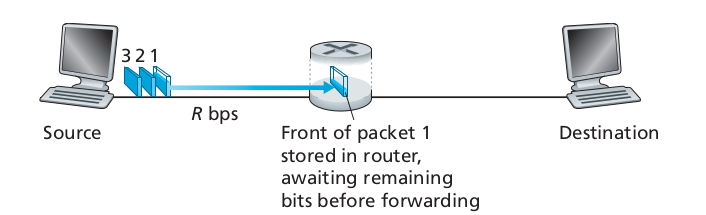
\includegraphics[width=0.8\textwidth]{chapters/chapter1/StoreAndForward.png}
    \label{c1_store&forward}
\end{center}

\begin{enumerate}
    \item The packet switch must receive the entire packet before it can transmit it.
    \item Store: the switch buffer the packet's bits.
    \item Forward: transmit the packet onto the outbound link.
\end{enumerate}


\subsection{Queuing Delays and Packet Loss}

\begin{enumerate}
    \item Each node has an output buffer/queue.
    \item Each packet on the buffer wait for its turn to be transmitted.
    \item Queuing Delay: The time that packet waits in the buffer.
    \item Packet Loss: when buffer is completey full, the arriving packets will be dropped.
\end{enumerate}

\begin{figure}
    \centering
    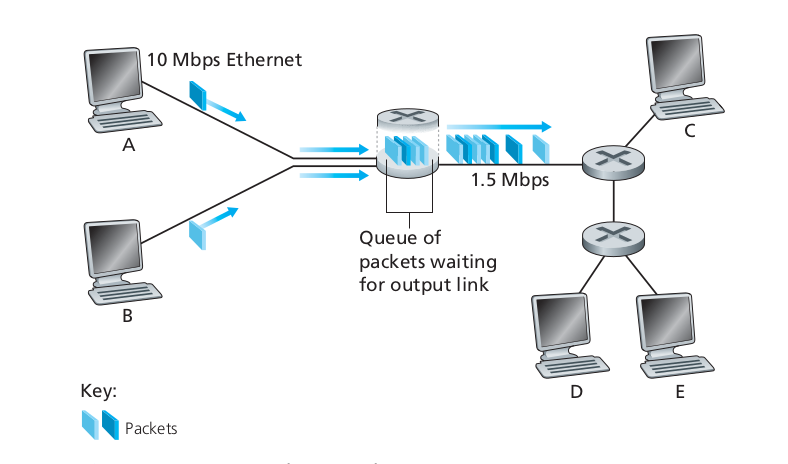
\includegraphics[width=0.6\textwidth]{chapters/chapter1/PacketSwitching.png}
    \caption{Packet Switching}
    \label{c1_packetSwitching}
\end{figure}

\subsection{Forwarding Tables and Routing Protocols}

\begin{enumerate}
    \item Each router has an IP address.
    \item Each router has a \textbf{forwarding table}: Maps the destination addresses to outbound links.
    \item End-to-end routing $<=>$ taxi driver who doesn't use map but instead prefers to ask the directions.
\end{enumerate}


\section{Circuit Switching}
Usage: traditional telephone networks.

\begin{enumerate}
    \item Circuit Switching reverse resources.
\end{enumerate}

\subsection{Multiplexing in Circuit-Switched networks}

\begin{enumerate}
    \item FDM: frequency-division multiplexing
    \item TDM: time-division multiplexing
\end{enumerate}

\subsubsection{FDM:frequency-division multiplexing}

Frequency spectrum of a link is divided up among the connections established across the link. \\
For example, FM radio stations use FDM to share frequency spectrum between 88MHZ nd 108MHZ.

\begin{figure}[!h]
    \centering
    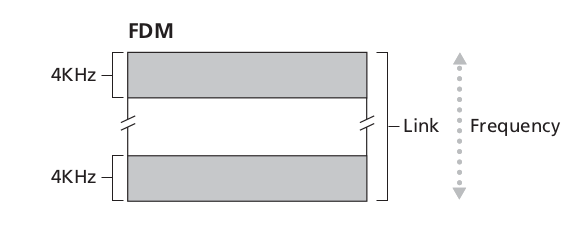
\includegraphics[width=0.4\textwidth]{chapters/chapter1/FDM.png}
    \caption{FDM}
    \label{c1_FDM}
\end{figure}


\subsubsection{TDM: time-division multiplexing}

Time is divided into frames of fixed duration, each frame is divided into fixed number of time slots.
Each frame is like a round. At each frame, the use has guaranteed time slots to use.

\begin{figure}[!h]
    \centering
    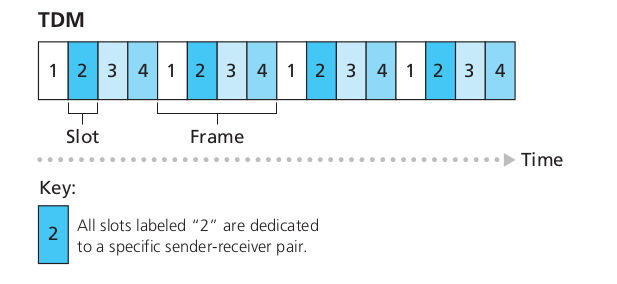
\includegraphics[width=0.4\textwidth]{chapters/chapter1/TDM.png}
    \caption{TDM}
    \label{c1_TDM}
\end{figure}




\subsection{Packet Switching Versus Circuit Switching}

\subsubsection{Advantage of Packet Switching}
\begin{enumerate}
    \item It offers better sharing of transmission capacity
    \item Simpler, more efficient, and less costly to implement.
\end{enumerate}

\subsection{Why Packet Switching is more efficient?}

Assumption: 90/10 rule: 90 percent of the time the user is idling.\\

Suppose users share a 1 Mbps link. Also suppose that each user alternates between peri-
ods of activity, when a user generates data at a constant rate of 100 kbps, and periods
of inactivity, when a user generates no data. Suppose further that a user is active
only 10 percent of the time.

With Circuit Switching, 100 kbps must be reversed even the user is drinking coffee. Therefore only 1Mbps/100Kps = 10
users can share the link at the same time.

With Packet Switching, if there are 35 users, the probability that there are 11 or more users using the link simultaneously is less
than 0.0004. Statistically, the packet switching is more efficient.

\subsection{Advantage of Circuit Switching}
\begin{enumerate}
    \item Rate is guaranteed, suitable for real time services.
\end{enumerate}


\subsection{Delay, Loss, and Throughput in Packet-Switched Networks}

Nodal delay = Processing Delay + Queuing Delay + Transmission Delay + Propagation Delay

\begin{figure}[!h]
    \centering
    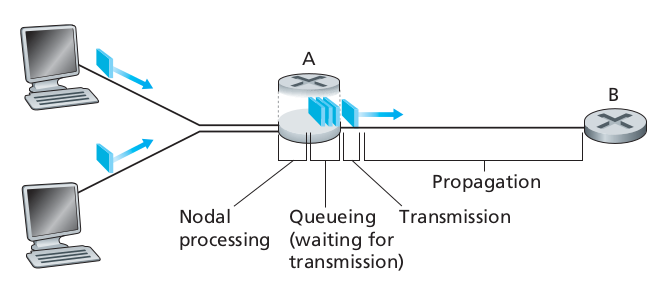
\includegraphics[width=0.6\textwidth]{chapters/chapter1/Delays.png}
\end{figure}

\begin{enumerate}
    \item Throughput: The amount of data per unit time that can be transferred between end hosts.
    \item Processing Delay: The time required to examine the packet's header and determine where to direct packet is part of processing delay.
    \item Queuing Delay: The time that the packet waits in the buffer.
    \item Transmission Delay: The amount of time to put the complete packet onto the link.
    \item Propagation Delay: The time required to propagate from the beginning of the link to the next node.
\end{enumerate}


\subsubsection{Processing Delay}
Several parts of the processing delay:
\begin{enumerate}
    \item The time required to examine the packet's header
    \item The time required to check bit-level errors
\end{enumerate}


\subsubsection{Queuing Delay}
The length of queuing delay is depended on the number of packets waiting in the buffer/queue. If the queue is empty and no other packet is currently
being transmitted, the queuing delay will be zero.\\
Queuing can vary in a large scope. Queuing
delays can be on the order of microseconds to milliseconds in practice.


\subsubsection{Transmission Delay}
Transmission delay depends on the physical medium of the link.\\
Transmission delay = the time the first bit is put on the link - the time the last bit is put on the link.
Denote the packet size L, and the transmission rate R.\\
The transmission delay will be $\frac{L}{R}$.

\subsubsection{Propagation Delay}
Propagation Delay depends on the physical medium of the link.\\
Denote the distanct between nodes d, and the speed of propagation (the speed of the link, usually a little less than the speed of light).\\
The propagation delay is d/s.\\
The progation delay can be negligible using fiber, but can be dominant if using satellite link.

\subsection{Queuing Delay and Packet Loss}
Unlike other delays, queuing delay can vary from packet to packet. For example 10 packets arrive at the same empty queue at the same time,
the first packet will have zero queuing delay and the last packet will have relatively large queuing delay.\\
When is the queuing delay large and when is it insignificant? => Depends on the rate of the arrving traffic(packets), the transmission rate
of the link, and hether the traffic arrives periodically or arrives in bursts.\\

Let a denote the average
rate at which packets arrive at the queue (a is in units of packets/sec). Recall that R is
the transmission rate; that is, it is the rate (in bits/sec) at which bits are pushed out of
the queue. Also suppose, for simplicity, that all packets consist of L bits.\\

\begin{center}
    Traffic instensity: $\frac{La}{R}$
\end{center}

If $\frac{La}{R} >1 $, the link is very busy and the queuing delay will continously increse and into infinite. If $\frac{La}{R} < 1$, is a necessary
for reduce the queuing delay.

\begin{figure}[!h]
    \centering
    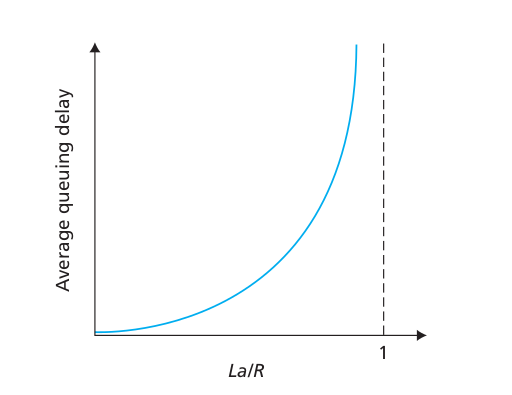
\includegraphics[width=0.5\textwidth]{chapters/chapter1/Queuing_delay.png}
    \caption{Dependence of average queuing delay on traffic intensity}
    \label{c1_queuingDelay_trafficIntensity}
\end{figure}


\subsection{End-to-End Delay}
Suppose there are $N-1$ routers between the source host and
the destination host. The transmission rate is fixed R, and the the distanct between each router is L.
The end-to-end delay is:
\begin{center}
    $d_{end-end} = \sum_{i=1}^N d_{proc}+d_{trans}+d_{prop}+d_{queu_i}$
\end{center}

\section{Protocol layering}

Five-layer Internet Protocol Stack: Each layer provides services to the layer aboves it by 1)performing certain actions within that layer and by
2)using the services of the layer directly below it.


\begin{figure}[!h]
    \centering
    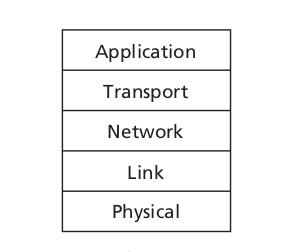
\includegraphics[width=0.3\textwidth]{chapters/chapter1/Layered.png}
    \caption{Five-layer Protocol Stack}
    \label{c1_protocol_stack}
\end{figure}

\subsection{Packet at different layers}
\begin{enumerate}
    \item Message : Application Layer
    \item Segment : Transport Layer
    \item Datagram : Network Layer
    \item Frame : Link Layer
\end{enumerate}

\subsection{Application Layer}
The Internet’s application layer includes many protocols:
\begin{enumerate}
    \item HTTP
    \item SMTP
    \item FTP
    \item DNS
    \item ...
\end{enumerate}

\subsection{Transport Layer}
\begin{enumerate}
    \item TCP
    \item UDP
\end{enumerate}

\subsection{Networking Layer}
Only one procotol is available at this layer => \textbf{IP} (\textit{Internet Protocol}).

\subsection{Link Layer}
Examples of linklayer protocols include:
\begin{enumerate}
    \item Ethernet
    \item WiFi
    \item DOCIS
\end{enumerate}

\subsection{Physical Layer}
The protocols in this layer are
again link dependent and further depend on the actual transmission medium of the
link
For example,
Ethernet has many physical-layer protocols:
\begin{enumerate}
    \item twisted-pair copper wire
    \item coaxial cable
    \item fiber
\end{enumerate}
In each case, a bit is moved
across the link in a different way.

\todo{Materials need to be learned}

\section{Encapsulation}

\begin{figure}[!h]
    \centering
    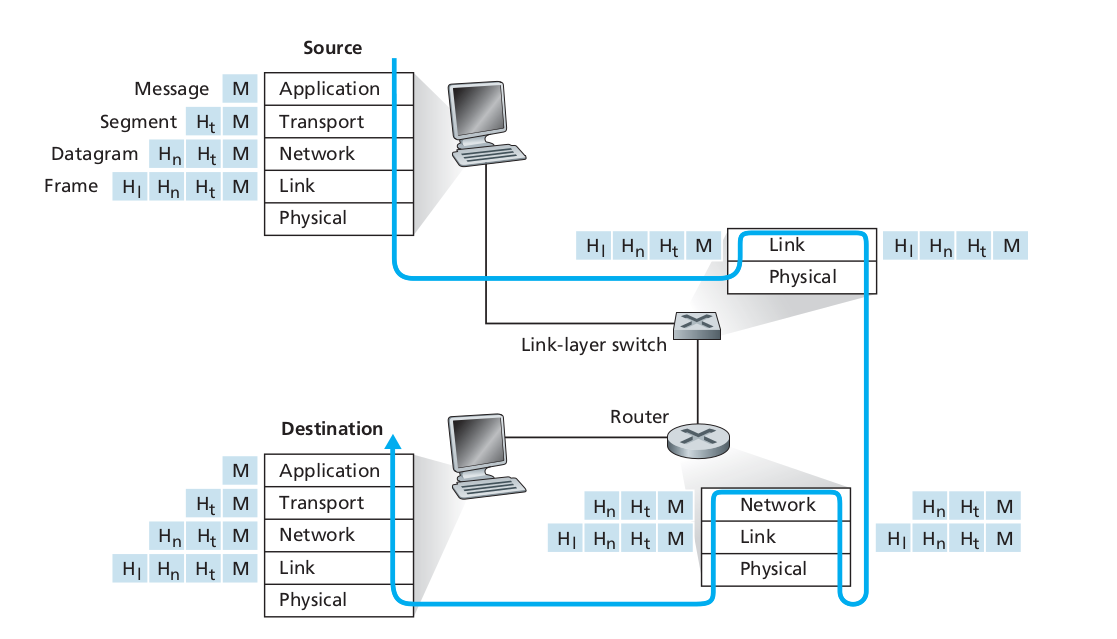
\includegraphics[width=0.8\textwidth]{chapters/chapter1/Encapsulation.png}
    \caption{Encapsulation}
    \label{c1_encapsulation}
\end{figure}